

\section{The homotopy theory of DG-algebras}

When we looked at some examples of model categories, we mentioned that the model structure on the category of DG-algebras would be similar to the model structure on unbounded chain complexes of modules over a ring. The model structure on $DGA_k$ was first constructed by Jardine in \cite{jardine}, and is described by the weak equivalences\index{Weak equivalence} being the quasi-isomorphisms\index{Quasi-isomorphism}, the fibrations\index{Fibration} being the degreewise surjections and the cofibrations\index{Cofibration} being all maps that have the left lifting property with respect to acyclic fibrations. 

Let's prove that this is in fact a model structure on the category $DGA_k$. Note that this construction---and proof---holds more generally for $k$ a commutative unital ring. The greater part of the proof below is directly inspired by the  original paper \cite{jardine}, but we have tried to fill in some details, and prove some parts that is left out by Jardine. We will not prove that the second factorization in \textbf{MC4} holds in $DGA_k$, as it requires us to go into the so-called ``small objects argument''. For a proof of that result, see \cite[Theorem 2.1.14]{hovey}, and for a more in depth conceptual treatment, see \cite{small_objects}.

To help us with some of the proofs of the different axioms we let:
\begin{itemize}
	\item $S(x)$ be the free graded $k$-algebra on one generator $x$ in degree $n$, together with the differential defined by $d(x)=0$.
	
	\item $T(x)$ be the free graded $k$-algebra on two generators, $x$ and $dx$, together with the differential defined by $d(x)=dx$ and $d(dx)=0$. This is the free DG-algebra on one generator.
	\item $C(x)$ be the free cochain complex on one generator $x$ in degree $n$, i.e. the complex 
\begin{equation*}
    C(x)^i = 
    \begin{cases}
        &  0, i\neq n, i\neq n+1 \\
        & k, i = n, i= n+1
    \end{cases}
\end{equation*}
where the differential is trivial, except for being the identity on $k$ in degree $n$. 
\end{itemize}


The \emph{coproduct of two DG-algebras}\index{Coproduct of DG-algebras}, $A$ and $B$, is defined by $A\ast B = T(A\otimes B)/I$, where $T(A\otimes B)$ is the tensor algebra
\begin{equation*}
    T(A\otimes B) = \bigoplus_{n \in \N}(A\otimes B)^{\otimes n}
\end{equation*}
and $I$ is the ideal generated by 
\begin{equation*}
	(a\otimes b_1)\otimes (1\otimes b_2) - a\otimes b_1 b_2, \quad (a_1\otimes 1)\otimes (a_2 \otimes b) - a_1 a_2 \otimes b.
\end{equation*}

Note that we can identify $T(x)$ with the tensor algebra on $C(x)$, i.e. 
\begin{equation*}
    T(x) \overset{\cong}\longrightarrow T(C(x)) = \bigoplus_{i\geq 0}C(x)^{\otimes i}
\end{equation*}

Hence we have 
\begin{equation*}
H^i(T(x)) = 
\begin{cases}
    &k, \quad i=0 \\
    &0, \quad \text{else}
\end{cases}
\end{equation*}

\begin{definition}
Let $A$ be a DG-algebra and $C$ a cochain complex. We define the DG-algebra $A[C]$ to be the cochain complex
\begin{equation*}
    A[C] = A\oplus (A\otimes C\otimes A) \oplus (A\otimes C \otimes A \otimes C \otimes A) \oplus \cdots
\end{equation*}
together with multiplication defined by 
\begin{equation*}
    (a_1\otimes b_1 \otimes \cdots \otimes b_k \otimes a_{k+1}) \cdot (a'_1\otimes b'_1 \otimes \cdots \otimes b'_l \otimes a'_{l+1}) = a_1 \otimes \cdots \otimes b_k \otimes a_{k+1}a'_1 \otimes \cdots \otimes b'_l \otimes a'_{l+1}
\end{equation*}
\end{definition}

For the sake of intuition we can---not completely accurately---think about this DG-algebra as a free algebra on $C$.

Any map from this DG-algebra $f:A[C]\longrightarrow B$ is uniquely determined by its restriction to its first component $A$, and the chain map on the first occurring $C$, i.e. the map $j_f$ defined by by the composition
\begin{equation*}
    j_f: C\overset{inc}\longrightarrow A\otimes C\otimes A \subseteq A[C]\overset{f}\longrightarrow B
\end{equation*}
where $inc(c) = 1\otimes c \otimes 1$. 

Hence we have an isomorphism $A\ast_k T(x) \cong A[C(X)]$ from the coproduct to this ``free algebra'' on $C$. This is because $T(x)\cong T(C(x))$, and the map $A[C(x)]\longrightarrow A\ast_k T(C(x))$ is uniquely determined by sending $A$ into $A$, and $C(x)$ into $C(x)$ as a component of $T(C(x))$. 


\begin{lemma}
The map $k\longrightarrow T(x)$ is a cofibration. 
\end{lemma}
\begin{proof}
We need to show that a lift $h:T(X)\longrightarrow A$ exists for all commuting diagrams of the form
\begin{center}
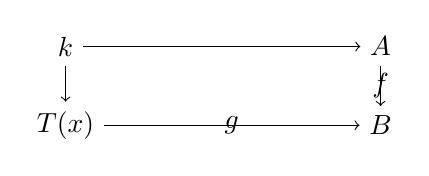
\begin{tikzpicture}
	\node (1) {$k$};
	\node (2) [below of=1] {$T(x)$};
	\node (3) [node distance=4cm, right of=1] {$A$};
	\node (4) [below of=3] {$B$};

	\draw [-to] (1) to node {} (2);
	\draw [-to] (1) to node {} (3);
	\draw [-to] (2) to node [swap]{$g$} (4);
	\draw [-to] (3) to node {$f$} (4);	
\end{tikzpicture}
\end{center}
where $f\colon A\longrightarrow B$ is an acyclic fibration. 
    
The push-out of the diagram 
\begin{center}
\begin{tikzpicture}
	\node (1) {$k$};
	\node (2) [below of=1] {$T(x)$};
	\node (3) [node distance=4cm, right of=1] {$A$};

	\draw [-to] (1) to node {} (2);
	\draw [-to] (1) to node {} (3);
\end{tikzpicture}
\end{center}
is the coproduct $A\ast_k T(x)$, which we know is isomorphic to $A[C(x)]$. Hence we have a unique map $B\longrightarrow A[C(x)]$ by the universal property of a push-out, i.e. 
\begin{center}
\begin{tikzpicture}
	\node (1) {$k$};
	\node (2) [below of=1] {$T(x)$};
	\node (3) [node distance=4cm, right of=1] {$A$};
	\node (4) [below of=3] {$B$};
	\node (5) [node distance=2cm, right of=4, below of=4] {$A[C(x)]$};

	\draw [-to] (1) to node {} (2);
	\draw [-to] (1) to node {} (3);
	\draw [-to] (2) to node [swap]{$g$} (4);
	\draw [-to] (3) to node {$f$} (4);	
	\draw [-to, dotted] (4) to node {$\phi$} (5);
	\draw [-to, bend left] (3) to node {} (5);
	\draw [-to, bend right] (2) to node {} (5);
\end{tikzpicture}
\end{center}
We can then define the map $h = p_A \circ \phi \circ g$, where $p_A$ is the projection onto the first component, which is uniquely determined by being the identity on $A$ and $j_{p_A} = 0$. 
    
Then the diagram 
\begin{center}
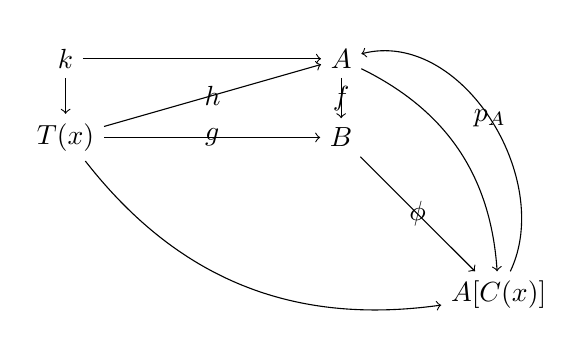
\begin{tikzpicture}
	\node (1) {$k$};
	\node (2) [below of=1] {$T(x)$};
	\node (3) [node distance=3.5cm, right of=1] {$A$};
	\node (4) [below of=3] {$B$};
	\node (5) [node distance=2cm, right of=4, below of=4] {$A[C(x)]$};

	\draw [-to] (1) to node {} (2);
	\draw [-to] (1) to node {} (3);
	\draw [-to] (2) to node [swap]{$g$} (4);
	\draw [-to] (3) to node {$f$} (4);	
	\draw [-to] (2) to node {$h$} (3);
	\draw [-to] (4) to node {$\phi$} (5);
	\draw [-to, bend left] (3) to node {} (5);
	\draw [-to, bend right] (2) to node {} (5);
	\draw [-to, bend right, in=250, out=300] (5) to node [swap]{$p_A$} (3);
\end{tikzpicture}
\end{center}
commutes everywhere, which means we have our desired lift $h$. 
\end{proof}


\begin{theorem}
\label{thm:dgak_model_category}
The category $DGA_k$ of DG-algebras over a field $k$, together with the three classes of morphisms; $W$, $C$, $F$, as described above, form a model category.
\end{theorem}

\begin{proof}
We need to check the four axioms. 

\textbf{MC 1:} This point consists of three sub-points. We first prove that $F$ is retraction closed\index{Retraction closed}, then $W$ and finally $C$. 

Assume $f:A\longrightarrow B$ is a retract of $g:X\longrightarrow Y$ where $g\in F$. This means we have a diagram

\begin{center}
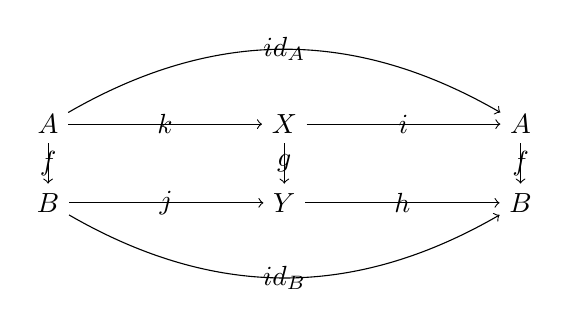
\begin{tikzpicture}
	\node (1) {$A$};
	\node (2) [below of=1] {$B$};
	\node (3) [node distance=3cm, right of=1] {$X$};
	\node (4) [below of=3] {$Y$};
	\node (5) [node distance=3cm, right of=3]{$A$};
	\node (6) [below of=5] {$B$};
	
	\draw [-to] (1) to node [swap]{$f$} (2);
	\draw [-to] (1) to node [swap]{$k$} (3);
	\draw [-to] (2) to node {$j$} (4);
	\draw [-to] (3) to node {$g$} (4);
	\draw [-to] (5) to node {$f$} (6);
	\draw [-to] (4) to node {$h$} (6);
	\draw [-to] (3) to node [swap]{$i$} (5);
	\draw [-to, bend left] (1) to node {$id_A$} (5);
	\draw [-to, bend right] (2) to node [swap] {$id_B$} (6);	
\end{tikzpicture}
\end{center}

Let $b$ be a homogeneous element in degree $n$. Want to show that there is a homogeneous element $a$ such that $f(a)=b$, as this would show that $f$ is degree-wise surjective, i.e. $f\in F$. 
    
Let $y = j(b)$. Since $g\in F$ it is a degree-wise surjection and hence there exists an element $x\in X$ such that $g(x)=y$. Let $i(x)=a$. Then we have 
\begin{align*}
    f(a) 
    &= f(i(x) \\
    &= h(g(x)) \\
    &= h(j(b)) \\
    &= id_B(b) = b.
\end{align*}
which shows that the retract of a fibration is again a fibration. 

For the second part we let $g\in W$ and $f$ still a retraction of $g$. We have the same retraction diagram as above, which induces the following diagram in cohomology:
\begin{center}
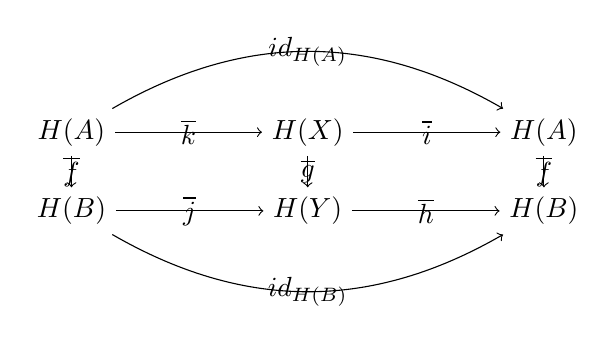
\begin{tikzpicture}
	\node (1) {$H(A)$};
	\node (2) [below of=1] {$H(B)$};
	\node (3) [node distance=3cm, right of=1] {$H(X)$};
	\node (4) [below of=3] {$H(Y)$};
	\node (5) [node distance=3cm, right of=3]{$H(A)$};
	\node (6) [below of=5] {$H(B)$};
	
	\draw [-to] (1) to node [swap]{$\overline{f}$} (2);
	\draw [-to] (1) to node [swap]{$\overline{k}$} (3);
	\draw [-to] (2) to node {$\overline{j}$} (4);
	\draw [-to] (3) to node {$\overline{g}$} (4);
	\draw [-to] (5) to node {$\overline{f}$} (6);
	\draw [-to] (4) to node {$\overline{h}$} (6);
	\draw [-to] (3) to node [swap]{$\overline{i}$} (5);
	\draw [-to, bend left] (1) to node {$id_{H(A)}$} (5);
	\draw [-to, bend right] (2) to node [swap] {$id_{H(B)}$} (6);	
\end{tikzpicture}
\end{center}

Recall that we want to show that $f$ induced an isomorphism in cohomology. As $g$ is surjective, we can use the same argument as above---when we had $f\in F$---to get that $\overline{f}$ is surjective. For injectivity we assume that $\overline{f}([a]) = \overline{f}([a'])$. Then $\overline{j}(\overline{f}([a])) = \overline{j}(\overline{f}([a']))$, which means $\overline{g}(\overline{k}([a])) = \overline{g}(\overline{k}([a']))$. But $\overline{g}$ is an isomorphism, and hence we have $\overline{k}([a]) = \overline{k}([a'])$, which finally gives us
\begin{equation*}
    [a] = id_A([a]) = \overline{i}(\overline{k}([a])) = \overline{i}(\overline{k}([a'])) = id_A([a']) = [a']
\end{equation*}
This shows that $\overline{f}$ is both injective and surjective, i.e. an isomorphism---which means that $f\in W$. 

For the last part we let $g\in C$, and $f$ still a retraction of $g$. Recall that we need to have a lift of $f$ with respect to all acyclic fibrations $[p\colon U\longrightarrow V]\in F\cap W$, i.e. the existence of the dotted morphism $\phi$ in the following diagram
\begin{center}
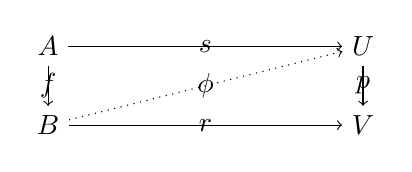
\begin{tikzpicture}
	\node (1) {$A$};
	\node (2) [node distance=4cm, right of=1] {$U$};
	\node (3) [below of=1] {$B$};
	\node (4) [below of=2] {$V$};

	\draw [-to] (1) to node {$s$} (2);
	\draw [-to] (1) to node [swap]{$f$} (3);
	\draw [-to] (2) to node {$p$} (4);
	\draw [-to] (3) to node [swap]{$r$} (4);	
	\draw [-to, dotted] (3) to node {$\phi$} (2);
\end{tikzpicture}
\end{center}

We get this by producing a lift from $g$. As $f$ is a retraction of $g$, we can extend the above diagram to 
\begin{center}
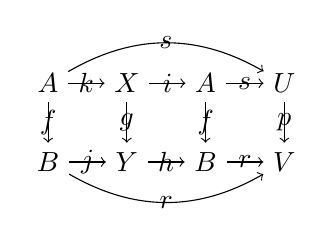
\begin{tikzpicture}
	\node (1) {$A$};
	\node (2) [right of=1] {$X$};	
	\node (3) [right of=2]{$A$};	
	\node (4) [right of=3] {$U$};	
	
	\node (5) [below of=1] {$B$};
	\node (6) [below of=2] {$Y$};
	\node (7) [below of=3] {$B$};
	\node (8) [below of=4] {$V$};
	
	\draw [-to] (1) to node [swap]{$f$} (5);
	\draw [-to] (1) to node [swap]{$k$} (2);
	\draw [-to] (5) to node {$j$} (6);
	\draw [-to] (2) to node {$g$} (6);
	\draw [-to] (3) to node {$f$} (7);
	\draw [-to] (6) to node {$h$} (7);
	\draw [-to] (2) to node [swap]{$i$} (3);
	\draw [-to] (3) to node [swap]{$s$} (4);
	\draw [-to] (7) to node {$r$} (8);	
	\draw [-to] (4) to node {$p$} (8);	
	\draw [-to, bend left] (1) to node {$s$} (4);
	\draw [-to, bend right] (5) to node [swap]{$r$} (8);	
\end{tikzpicture}
\end{center}

This diagram has the sub-diagram  
\begin{center}
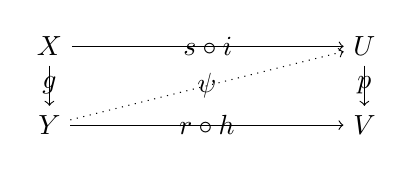
\begin{tikzpicture}
	\node (1) {$X$};
	\node (2) [node distance=4cm, right of=1] {$U$};
	\node (3) [below of=1] {$Y$};
	\node (4) [below of=2] {$V$};

	\draw [-to] (1) to node {$s\circ i$} (2);
	\draw [-to] (1) to node [swap]{$g$} (3);
	\draw [-to] (2) to node {$p$} (4);
	\draw [-to] (3) to node [swap]{$r\circ h$} (4);	
	\draw [-to, dotted] (3) to node {$\psi$} (2);
\end{tikzpicture}
\end{center}
where we know that the lift $\psi$, exists, as $g\in C$ and $p\in F\cap W$. We can then define $\psi = \psi\circ j$, i.e. the dotted arrow in the following diagram
\begin{center}
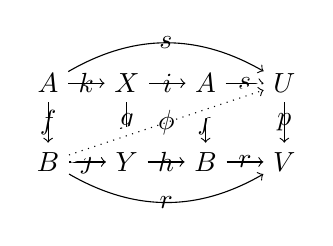
\begin{tikzpicture}[%
	cross line/.style={preaction={draw=white, -,line width=6pt}}]
	\node (1) {$A$};
	\node (2) [right of=1] {$X$};	
	\node (3) [right of=2]{$A$};	
	\node (4) [right of=3] {$U$};	
	
	\node (5) [below of=1] {$B$};
	\node (6) [below of=2] {$Y$};
	\node (7) [below of=3] {$B$};
	\node (8) [below of=4] {$V$};
	
	\draw [-to] (1) to node [swap]{$f$} (5);
	\draw [-to] (1) to node {$k$} (2);
	\draw [-to] (5) to node [swap]{$j$} (6);
	\draw [-to] (2) to node [swap]{$g$} (6);
	\draw [-to] (3) to node {$f$} (7);
	\draw [-to] (6) to node [swap]{$h$} (7);
	\draw [-to] (2) to node {$i$} (3);
	\draw [-to] (3) to node {$s$} (4);
	\draw [-to] (7) to node [swap]{$r$} (8);	
	\draw [-to] (4) to node {$p$} (8);	
	\draw [-to, bend left] (1) to node {$s$} (4);
	\draw [-to, bend right] (5) to node [swap]{$r$} (8);	
	\draw [-to, cross line, dotted] (5) to node {$\phi$} (4);
	
\end{tikzpicture}
\end{center}
Hence all retractions of morphisms in $C$ satisfy the lifting property with respect to morphisms in $F\cap W$, which means they are again in $C$. 


\textbf{MC 2:} Isomorphisms of DG-algebras have the two out of three property, and since quasi-isomorphisms are defined by inducing isomorphisms on the cohomology algebras, they also satisfy the property. 
    
\textbf{MC 3:} Notice that one half of this axiom holds by definition, as we defined cofibrations to be the morphisms that satisfied the left lifting property\index{Left lifting property} with respect to acyclic fibrations. For the other half we need to show that if we have a diagram 
\begin{center}
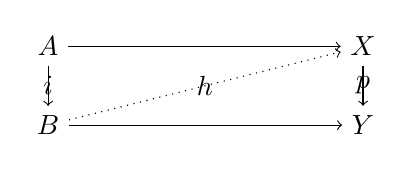
\begin{tikzpicture}
	\node (1) {$A$};
	\node (3) [below of=1] {$B$};
	\node (2) [node distance=4cm, right of=1] {$X$};
	\node (4) [below of=2] {$Y$};

	\draw [-to] (1) to node {} (2);
	\draw [-to] (1) to node [swap]{$i$} (3);
	\draw [-to] (2) to node {$p$} (4);
	\draw [-to] (3) to node [swap]{} (4);	
	\draw [-to, dotted] (3) to node {$h$} (2);
\end{tikzpicture}
\end{center}
where $i$ is an acyclic cofibration, and $p$ a fibration, then a lift $h$ exists. 
    
We can translate the problem to showing that every morphism $i\in C\cap W$ has the right lifting property\index{Right lifting property} w.r.t. all fibrations $p\in F$. 
    
Assume we have proven MC4, then we can factorize $i= f\circ j$ such that $j\in C\cap W$ and $f\in F$. Since two of them are in $W$, the last one also is by MC2.

Hence we have a diagram 
\begin{center}
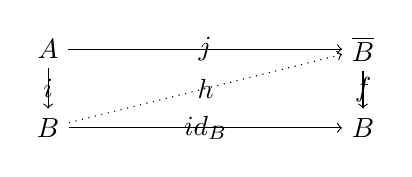
\begin{tikzpicture}
	\node (1) {$A$};
	\node (3) [below of=1] {$B$};
	\node (2) [node distance=4cm, right of=1] {$\overline{B}$};
	\node (4) [below of=2] {$B$};

	\draw [-to] (1) to node {$j$} (2);
	\draw [-to] (1) to node [swap]{$i$} (3);
	\draw [-to] (2) to node {$f$} (4);
	\draw [-to] (3) to node [swap]{$id_B$} (4);	
	\draw [-to, dotted] (3) to node {$h$} (2);
\end{tikzpicture}
\end{center}
    
that has a lift $h$ by the fact that $i\in C\cap W$ and $j\in F$. 

We use the commutativity of the previous diagram to get the new following diagram: 
\begin{center}
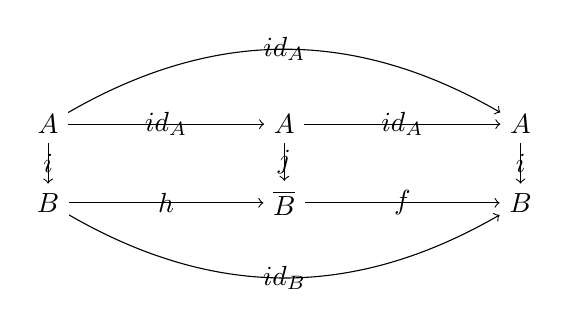
\begin{tikzpicture}
	\node (1) {$A$};
	\node (2) [below of=1] {$B$};
	\node (3) [node distance=3cm, right of=1] {$A$};
	\node (4) [below of=3] {$\overline{B}$};
	\node (5) [node distance=3cm, right of=3]{$A$};
	\node (6) [below of=5] {$B$};
	
	\draw [-to] (1) to node [swap]{$i$} (2);
	\draw [-to] (1) to node [swap]{$id_A$} (3);
	\draw [-to] (2) to node {$h$} (4);
	\draw [-to] (3) to node {$j$} (4);
	\draw [-to] (5) to node {$i$} (6);
	\draw [-to] (4) to node {$f$} (6);
	\draw [-to] (3) to node [swap]{$id_A$} (5);
	\draw [-to, bend left] (1) to node {$id_A$} (5);
	\draw [-to, bend right] (2) to node [swap] {$id_B$} (6);	
\end{tikzpicture}
\end{center}
This shows that $i$ is a retraction of $j$, which we know has the right lifting property w.r.t all maps $f\in F$, hence $i$ does as well by MC1.



\textbf{MC 4:} Let $f:A\longrightarrow B$ be any map between two DG-algebras. We can form the factorization 
\begin{equation*}
    A\overset{i}\longrightarrow A\ast (\ast_{b\in B} T(B))\overset{p}\longrightarrow B
\end{equation*}
where $i$ is the inclusion and $p$ is the map that sends the generator $b \in T(B)$ to $b\in B$. The map $q$ is a fibration as it is  degreewise surjection, and the map $i$ is a filtered colimit of maps $A\longrightarrow T(b_1)\ast \cdots T(b_n)\ast A$, which all are acyclic cofibrations by iterating the construction of the isomorphism $T(x)\ast A \cong A[C(x)]$ we saw earlier. Hence it is also itself an acyclic cofibration. 

The last factorization is as mentioned left out, due to us not covering the small objects argument in this thesis. See \cite[Lemma 3]{jardine} for a proof using this argument. 
\end{proof}


As we now know that $DGA_k$ is a model category, we know there exists a terminal and an initial object. In $DGA_k$ the terminal object is $0$---the complex consisting only of zeroes with only trivial differentials and trivial multiplication---while the initial object is the ground field $k$---treated as a DG-algebra by having only one copy of $k$ in degree zero and zeroes everywhere else. Since the unique map $A\longrightarrow 0$ is a degreewise surjection for any DG-algebra $A$ we know that all DG-algebras are fibrant objects\index{Fibrant object} in this model structure. 




\subsection{More formality}

This new framework allows us to reconsider the definition of a formal DG-algebra. We take the category $DGA_k$, which we now know is a model category with $W$ being the collection of quasi-isomorphisms, and produce its homotopy category $HoDGA_k = DGA_k[W^{-1}]$. We can then define a DG-algebra to be formal as follows. 

\begin{definition}[Formal DG-algebra]
\label{def:formal_dga2}
\index{Formal DG-algebra}
A DG-algebra $(A, d)$ is called formal if it is isomorphic to its cohomology algebra $H(A)$ in $HoDGA_k$.
\end{definition}

This is the precise reason we in the abstract referred to formal DG-algebras as being the algebras that contain the same homotopical information as their cohomology algebra. They are isomorphic in the homotopy category, hence contain the same information up to homotopy, e.g. homotopical information. 

Unfortunately not all isomorphisms in $HoDGA_k$ come from a single quasi-isomorphism in $DGA_k$. Quasi-isomorphisms in $DGA_k$ are not invertible in general---not even invertible up to homotopy. Thus a zig-zag of quasi-isomorphisms is the best we can hope for, which means that this new definition is precisely the same as the old. 

A feature of this new framework is that we actually don't need an arbitrary zig-zag of quasi-isomorphisms---we only need a single span. A \emph{span of morphisms}\index{Span of morphisms} is a diagram of the following form:

\begin{center}
\begin{tikzpicture}
	\node (1) {$A$};
	\node (2) [right of=1] { };	
	\node (3) [right of=2] {$B$};	
	\node (4) [node distance=1cm, above of=2] {$C$};

	\draw [-to] (4) to node [swap]{} (1);
	\draw [-to] (4) to node {} (3);
\end{tikzpicture}
\end{center}

If we reverse the directions of the two arrows we get a diagram called a \emph{cospan}\index{Cospan of morphisms}. To prove this we will need the following. 

\begin{definition}[Right proper model category]
\label{def:right_proper}
\index{Right proper model category}
Let $\C$ be a model category. We say it is right proper if the pullback of a weak equivalence along a fibration is again a weak equivalence. 
\end{definition}

As a consequence of the fact that all objects in $DGA_k$ are fibrant, and the fact that pullbacks of weak equivalences along fibrations between fibrant objects is again a weak equivalence, we have that $DGA_k$---with the model structure defined above---is a right proper model category.  

\begin{theorem}
\label{thm:span}
Let $A$ and $B$ be quasi-isomorphic DG-algebras\index{Quasi-isomorphic DG-algebras}. Then there exists a DG-algebra $C$ and two quasi-isomorphisms $q_1, q_2$ such that $A\overset{q_1}\longleftarrow C \overset{q_2}\longrightarrow B$
\end{theorem}
\begin{proof}
Since we know $A$ and $B$ are quasi-isomorphic, we have a zig-zag of quasi-isomorphisms between them. Assume this sequence has length $r$. There are four possible ways this zig-zag can look at its ends. On the left we can have either a quasi-isomorphism $A\longrightarrow A_1$, or $A\longleftarrow A_1$. Similarly on the other end we can have either $A_r\longrightarrow B$ or $A_r\longleftarrow B$. 

Notice that if we prove that we can turn a cospan $A_{i-1}\longrightarrow A_i\longleftarrow A_{i+1}$ into a span $A_{i-1}\longleftarrow C_i \longrightarrow A_{i+1}$, then we have proved the theorem. This is due to composition of quasi-isomorphisms again being quasi-isomorphisms, which means that at the ends we get for example
\begin{center}
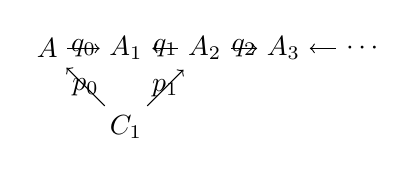
\begin{tikzpicture}
	\node (1) {$A$};
	\node (2) [right of=1] {$A_1$};
	\node (3) [right of=2] {$A_2$};
	\node (4) [right of=3] {$A_3$};
	\node (5) [right of=4] {$\cdots$};
	\node (6) [below of=2] {$C_1$};
	
	\draw [-to] (1) to node {$q_0$} (2);
	\draw [to-] (2) to node {$q_1$} (3);
	\draw [-to] (3) to node {$q_2$} (4);
	\draw [to-] (4) to node {} (5);
	\draw [-to] (6) to node {$p_0$} (1);
	\draw [-to] (6) to node [swap]{$p_1$} (3);	
\end{tikzpicture}
\end{center}
By composing $p_2$ and $q_2$, the length of the zig-zag is reduced to $r-1$. Hence we can iterate this for all the cospans in the zig-zag, and the end result will be a simple nice span. 

So, let's assume we have a cospan $A_{i-1}\overset{q_{i-1}}\longrightarrow A_i\overset{q_i}\longleftarrow A_{i+1}$. We could take its pullback, but we have no justification for saying that the maps in the pullback are again quasi-isomorphisms, but---as $DGA_k$ is right proper---we know that pullback of a weak equivalence along a fibration is again a weak equivalence. By \textbf{MC4} we know that the quasi-isomorphisms $q_{i-1}$ and $q_i$ can be factorized as $q_{i-1} = i \circ q$ and $q_i = j\circ p$, where $q, p$ are cofibrations and $i, j$ are acyclic fibrations. By the two-out-of-three property of weak equivalences, we also know that $q, p$ are acyclic cofibrations. This means we have the following diagram
\begin{center}
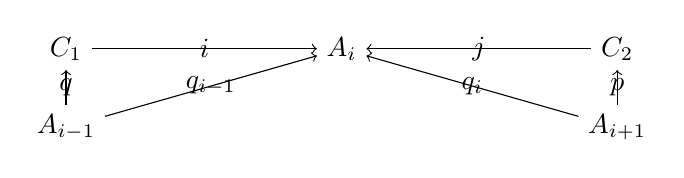
\begin{tikzpicture}
	\node (1) {$C_1$};
	\node (2) [node distance=3.5cm, right of=1] {$A_i$};
	\node (3) [node distance=3.5cm, right of=2] {$C_2$};
	\node (4) [below of=1] {$A_{i-1}$};
	\node (5) [below of=3] {$A_{i+1}$};
	
	\draw [-to] (1) to node {$i$} (2);
	\draw [to-] (2) to node {$j$} (3);
	\draw [-to] (4) to node [swap]{$q_{i-1}$} (2);
	\draw [-to] (5) to node {$q_i$} (2);
	\draw [-to] (4) to node {$q$} (1);
	\draw [-to] (5) to node [swap]{$p$} (3);		
\end{tikzpicture}
\end{center}
for some DG-algebras $C_1$ and $C_2$. Consider now the diagram
\begin{center}
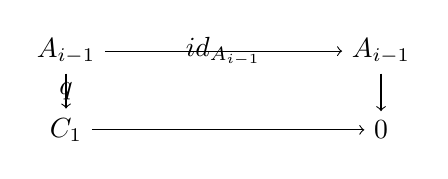
\begin{tikzpicture}
	\node (1) {$A_{i-1}$};
	\node (2) [node distance=4cm, right of=1] {$A_{i-1}$};	
	\node (3) [below of=1] {$C_1$};
	\node (4) [below of=2] {$0$};

	\draw [-to] (1) to node {$id_{A_{i-1}}$} (2);
	\draw [-to] (1) to node [swap]{$q$} (3);
	\draw [-to] (2) to node {} (4);
	\draw [-to] (3) to node {} (4);	
\end{tikzpicture}
\end{center}
As all objects are fibrant we know that $A_{i-1}\longrightarrow 0$ is a fibration. By \textbf{MC3}  there exists a lift, $q'\colon C_1\longrightarrow A$ making the sub-diagrams commute. In particular $q'\circ q = id_{A_{i-1}}$. Since $q$ and $id_{A_{i-1}}$ are both quasi-isomorphisms, $q'$ has to be as well due to the two-out-of-three property. Similarily a quasi-isomorphism $p'$ exists such that $p'\circ p = id_{A_{i+1}}$. 

The next step is to take the pullback of the cospan $C_1\overset{i}\longrightarrow A_i\overset{j}\longleftarrow C_2$, i.e.
\begin{center}
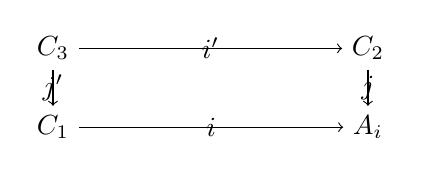
\begin{tikzpicture}
	\node (1) {$C_3$};
	\node (2) [node distance=4cm, right of=1] {$C_2$};	
	\node (3) [below of=1] {$C_1$};
	\node (4) [below of=2] {$A_i$};

	\draw [-to] (1) to node {$i'$} (2);
	\draw [-to] (1) to node [swap]{$j'$} (3);
	\draw [-to] (2) to node {$j$} (4);
	\draw [-to] (3) to node [swap]{$i$} (4);	
\end{tikzpicture}
\end{center}
As $i$ and $j$ are both acyclic fibrations, the maps $i'$ and $j'$ will be as well. This is because being a fibration is stable under pullback, and being a quasi-isomorphism is stable when we are pulling back along a fibration---which both maps are. Now we have a diagram

\begin{center}
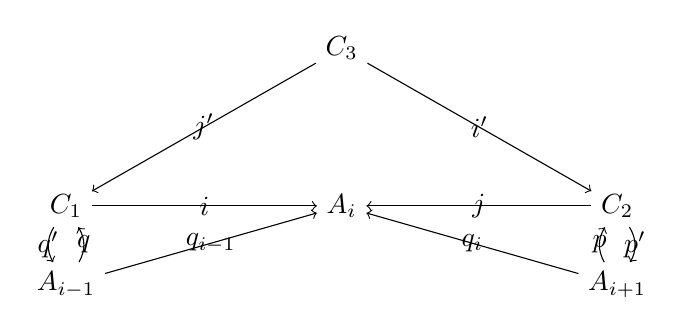
\begin{tikzpicture}
	\node (1) {$C_1$};
	\node (2) [node distance=3.5cm, right of=1] {$A_i$};
	\node (3) [node distance=3.5cm, right of=2] {$C_2$};
	\node (4) [below of=1] {$A_{i-1}$};
	\node (5) [below of=3] {$A_{i+1}$};
	\node (6) [node distance=2cm, above of=2] {$C_3$};
	
	\draw [-to] (6) to node [swap]{$j'$} (1);
	\draw [-to] (6) to node {$i'$} (3);
	\draw [-to] (1) to node {$i$} (2);
	\draw [to-] (2) to node {$j$} (3);
	\draw [-to] (4) to node [swap]{$q_{i-1}$} (2);
	\draw [-to] (5) to node {$q_i$} (2);
	\draw [-to, bend right] (4) to node [swap]{$q$} (1);
	\draw [-to, bend left] (5) to node {$p$} (3);	
	\draw [to-, bend left] (4) to node {$q'$} (1);
	\draw [to-, bend right] (5) to node [swap]{$p'$} (3);				
\end{tikzpicture}
\end{center}

And the compositions $q'\circ i'$ and $p'\circ j'$ are both quasi-isomorphisms, as all four individually are. Hence we have a span $A_{i-1}\longleftarrow C_3 \longrightarrow A_{i+1}$, which by the argument above means we can reduce any zig-zag of quasi-isomorphisms $A\longleftarrow \cdots \longrightarrow B$ to a single span $A\longleftarrow C\longrightarrow B$, for some DG-algebra $C$. 
\end{proof}

This finally resolves \textbf{Theorem A.} from the motivation in the beginning of this chapter. We have a formal DG-algebra if and only if there is a span of quasi-isomorphisms connecting it to its cohomology.  


We didn't actually use the specific model structure on $DGA_k$ in this proof, so the same argument holds for any right proper model categories where all objects are fibrant. 

Notice that this also implies that $DGA_k$ satisfies the \emph{right Ore condition}\index{The right Ore condition}, i.e. that given a cospan $A\overset{a}\longrightarrow C \overset{q}\longleftarrow B$, where $q$ is a quasi-isomorphism, then there exists a span $A\overset{q'}\longleftarrow C' \longrightarrow B$ where $q'$ is a quasi-isomorphism. This follows from the proof above as we can factorize $a$ into $f\circ c$, where $c$ is an acyclic cofibration and $f$ a fibration. We can take the pullback of $D\longrightarrow C\longleftarrow B$ to get the diagram
\begin{center}
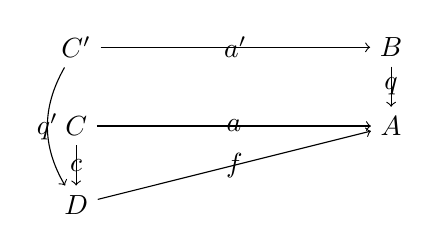
\begin{tikzpicture}
	\node (1) {$C'$};
	\node (2) [node distance=4cm, right of=1] {$B$};	
	\node (3) [below of=1] {$C$};
	\node (4) [below of=2] {$A$};
	\node (5) [below of=3] {$D$};

	\draw [-to] (1) to node {$a'$} (2);
	\draw [-to, bend right] (1) to node [swap]{$q'$} (5);
	\draw [-to] (2) to node {$q$} (4);
	\draw [-to] (3) to node [swap]{$a$} (4);
	\draw [-to] (3) to node {$c$} (5);
	\draw [-to] (5) to node [swap]{$f$} (4);
\end{tikzpicture}
\end{center}
where now $q'$ is a quasi-isomorphism, as it is a pullback of a quasi-isomorphism along the fibration $f$. As in the previous proof---because $A$ is fibrant---we get a left inverse to the acyclic cofibration $c$, which is again a quasi-isomorphism. This is the lift we get from the following diagram
\begin{center}
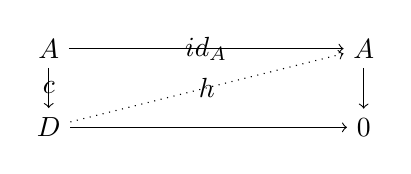
\begin{tikzpicture}
	\node (1) {$A$};
	\node (2) [node distance=4cm, right of=1] {$A$};	
	\node (3) [below of=1] {$D$};
	\node (4) [below of=2] {$0$};

	\draw [-to] (1) to node {$id_A$} (2);
	\draw [-to] (1) to node [swap]{$c$} (3);
	\draw [-to] (2) to node {} (4);
	\draw [-to] (3) to node {} (4);	
	\draw [-to, dotted] (3) to node {$h$} (2);
\end{tikzpicture}
\end{center}
Denote this lift by $c'$. We now have the final diagram
\begin{center}
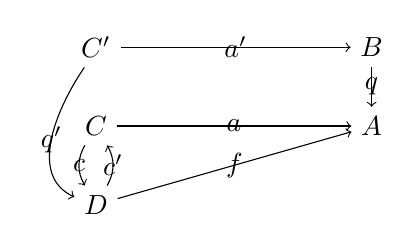
\begin{tikzpicture}
	\node (1) {$C'$};
	\node (2) [node distance=3.5cm, right of=1] {$B$};	
	\node (3) [below of=1] {$C$};
	\node (4) [below of=2] {$A$};
	\node (5) [below of=3] {$D$};

	\draw [-to] (1) to node {$a'$} (2);
	\draw [-to, bend right, in=250] (1) to node [swap]{$q'$} (5);
	\draw [-to] (2) to node {$q$} (4);
	\draw [-to] (3) to node [swap]{$a$} (4);
	\draw [-to, bend right] (3) to node [swap]{$c$} (5);
	\draw [to-, bend left] (3) to node {$c'$} (5);	
	\draw [-to] (5) to node [swap]{$f$} (4);
\end{tikzpicture}
\end{center}
where by the composition $c'\circ q'$---which is a quasi-isomorphism---we get our wanted span $A\overset{c'\circ q'}\leftarrow C'\rightarrow B$. 

This Ore condition allows the homotopy category $HoDGA_k$ to be described even more explicitly using spans as the morphisms. This means that a morphism $A\longrightarrow B$ is given by a span
\begin{center}
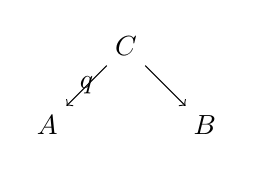
\begin{tikzpicture}
	\node (1) {$A$};
	\node (2) [right of=1] { };	
	\node (3) [right of=2] {$B$};	
	\node (4) [node distance=1cm, above of=2] {$C$};

	\draw [-to] (4) to node [swap]{$q$} (1);
	\draw [-to] (4) to node {} (3);
\end{tikzpicture}
\end{center}
where $q$ is a quasi-isomorphism. Composition of morphisms $A\longrightarrow B$ and $B\longrightarrow C$ is then given as
\begin{center}
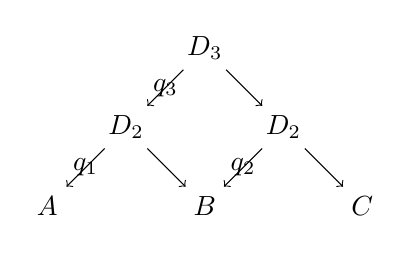
\begin{tikzpicture}
	\node (1) {$A$};
	\node (2) [right of=1] {};	
	\node (3) [right of=2] {$B$};	
	\node (4) [node distance=1cm, above of=2] {$D_2$};
	\node (5) [right of=3] {};
	\node (6) [right of=5] {$C$};
	\node (7) [node distance=1cm, above of=5] {$D_2$};
	\node (8) [right of=4] {};
	\node (9) [node distance=1cm, above of=8] {$D_3$};

	\draw [-to] (4) to node [swap]{$q_1$} (1);
	\draw [-to] (4) to node {} (3);
	\draw [-to] (7) to node [swap]{$q_2$} (3);
	\draw [-to] (7) to node {} (6);	
	\draw [-to] (9) to node [swap]{$q_3$} (4);
	\draw [-to] (9) to node {} (7);		
\end{tikzpicture}
\end{center}
where $q_3$ exists due to the Ore condition. As $q_3\circ q_1$ is again a quasi-isomorphism, we have a new span
\begin{center}
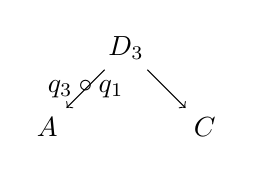
\begin{tikzpicture}
	\node (1) {$A$};
	\node (2) [right of=1] { };	
	\node (3) [right of=2] {$C$};	
	\node (4) [node distance=1cm, above of=2] {$D_3$};

	\draw [-to] (4) to node [swap]{$q_3\circ q_1$} (1);
	\draw [-to] (4) to node {} (3);
\end{tikzpicture}
\end{center}

We won't need, or use, this fact during the thesis, but it is a nice interesting consequence of the results in the chapter. It is also nice to know that $DGA_k$ has a nice homotopy category, as we have already described our main interest---formality---by being a consequence of isomorphisms in this homotopy category\index{The homotopy category}. 



% \begin{definition}{Homotopy}
% Let $f, g:A\longrightarrow B$ be two DG morphisms. A homotopy $h:f\rightarrow g$ is a map $h:A\longrightarrow B$ such that 
% \begin{itemize}
%     \item $g-f = d_B h + h d_A$
%     \item $h m_A = m_B(f\otimes h + h\otimes g)$
% \end{itemize}
% \end{definition}
% This is definition 4.3. in Proute french thesis
